\documentclass[10pt,a4paper]{article}
\usepackage[utf8]{inputenc}
\usepackage[spanish]{babel}
\usepackage{amsmath}
\usepackage{amsfonts}
\usepackage{amssymb}
\usepackage{enumitem}
\usepackage{hyperref} 
\usepackage{graphicx}
\usepackage[left=1in,right=1in]{geometry}
\hypersetup{pdftex,colorlinks=true,allcolors=blue}
\hypersetup{
    pdftitle={},
    pdfauthor={Pablo Riutort Grande},
    pdfsubject={},
    bookmarksnumbered=true,     
    bookmarksopen=true,         
    bookmarksopenlevel=1,       
    colorlinks=true,            
    pdfstartview=Fit,           
    pdfpagemode=UseOutlines,    % this is the option you were lookin for
    pdfpagelayout=TwoPageRight
}
\usepackage{listings}
\usepackage{xcolor}
\usepackage{hypcap}
\definecolor{codegreen}{rgb}{0,0.6,0}
\definecolor{codegray}{rgb}{0.5,0.5,0.5}
\definecolor{codepurple}{rgb}{0.58,0,0.82}
\definecolor{backcolour}{rgb}{0.95,0.95,0.92}
\lstdefinestyle{mystyle}{
    backgroundcolor=\color{backcolour},   
    commentstyle=\color{codegreen},
    keywordstyle=\color{magenta},
    numberstyle=\tiny\color{codegray},
    stringstyle=\color{codepurple},
    basicstyle=\ttfamily\footnotesize,
    breakatwhitespace=false,         
    breaklines=true,                 
    captionpos=b,                    
    keepspaces=true,                 
    numbers=left,                    
    numbersep=5pt,                  
    showspaces=false,                
    showstringspaces=false,
    showtabs=false,                  
    tabsize=2
}
\lstset{style=mystyle}
\usepackage{xparse}
\NewDocumentCommand{\codeword}{v}{%
\texttt{{#1}}
}

\author{Pablo Riutort Grande}
\title{PEC 1\\ \vspace{1cm}\textbf{Seguridad en Sistemas Operativos}}
\begin{document}
\maketitle
\pagebreak
\section{Linux}

\subsection{}

\begin{table}[htbp]
\resizebox{\textwidth}{!}{
\begin{tabular}{|l|l|c|}
\hline
 & \textbf{Comando} & \textbf{Valor} \\ \hline
 Versión del kernel & uname -r & 4.19.0-8-amd64 \\ \hline
 Num. particiones del disco & df -h  $\lvert$ grep \textasciicircum /dev $\lvert$ wc -l & 4 \\ \hline
 Memoria del sistema & head -1 /proc/meminfo & MemTotal:  4041712 kB  \\ \hline
 Servidor DNS configurado & cat /etc/resolv.conf $\lvert$ tail -1 & nameserver 10.0.2.3 \\ \hline
 Gateway de la subred & ip -br route show $\lvert$ head -1  & default via 10.0.2.2 dev enp0s3 proto dhcp metric 100 \\ \hline
 Dirección IP & ip -br addr show $\lvert$ tail -1 & 10.0.2.15/24 fe80::a00:27ff:fe23:3552/64 \\ \hline
 Tipo de sistema en / & df -h / - -output=fstype $\lvert$ tail -1 & ext4 \\ \hline
 Espacio utilizado en la / & df -h / - -output=used $\lvert$ tail -1 & 3.0G \\ \hline
\end{tabular}
}
\end{table}

\subsection{}
Creo que el sistema debería tener particiones para /var puesto que en este directorio se guardan los logs, emails y otros datos de sistemas de bases de datos. Un mejor esquema de pariticiones sería:
\begin{itemize}
\item /tmp
\item /var
\item /var/log
\item /var/www
\item /home
\item /usr
\end{itemize}
\subsection{}
Primero crearía una partición de disco con el comando fdisk. Este comando listar las particiones en disco (fdisk -l) y añadir nuevas tablas de partición (fdisk /dev/\textless sd\textgreater) y guardarlas en disco. Este se consigue con las opciones ''n'' para crear una nueva partición y seleccionamos el tipo con ''e'' y ''p'' (extendida o primaria). Los siguientes pasos tienen que ver con la configuración de la partición en sí, como el espacio que tendrá asignado.\\
Una vez hecho esto, con el comando mkfs se crea un sistema de ficheros en la partición, en nuestro caso: ''mkfs -t ext3 /dev/\textless sd\textgreater''  dará formato a la partición y creará un sistema de journal tipo ext3.\\
Finalmente podemos montar el sistema de ficheros con el comando ''mount'' y hacerlo persistente en el sistema modificando el archivo /etc/fstab.\\
Alternativamente, se puede realizar el mismo proceso instalando herramientas gráficas de particionado como GParted.
\subsection{}
Para mover /home a una nueva partición podemos usar el comando fdisk. Con fdisk -l podemos listar las particiones y discos. Supongamos que el comando lista un disco /dev/sdb, los pasos a realizar serían los siguientes:
\begin{enumerate}
\item Creamos una partición nueva con fdisk /dev/sdb de tipo primaria (opción n y despúes p).
\item Confirmamos la partición con ''w'' que nos creará la partición con nombre similar a /dev/sdb1.
\item Creamos el sistema de ficheros en la nueva partición con mkfs -t ext4 /dev/sdb1.
\item Montamos el nuevo disco con mount /dev/sdb1 /mnt (siendo /mnt nuestro punto de montaje). Esto nos permite copiar datos en el nuevo disco.
\item Movemos (o copiamos) el directorio /home en el punto de montaje: mv /home/* /mnt
\item Ahora podemos crear un nuevo directorio /home en nuestra raíz que será el punto de montaje del disco (que ahora contiene /home): mkdir /home.
\item Finalmente, montamos el disco en /home: umount /dev/sdb1; mount /dev/sdv1 /home/
\end{enumerate}

Mount the external partition onto a temporary Home location.\\
Copy the files from your current Home folder to this temporary Home folder.\\
Relocate the current Home folder\\
Mount the new Home folder.
\subsection{}
El siguiente comando crea un usuario con directorio propio en /home, fecha de expiración a 1/1/2018, bash como shell, perteneciente al grupo users y con nombre ''alumno''.
\begin{lstlisting}[language=bash]
sudo useradd -m -e 2018-01-01 -s /bin/bash -G users alumno
\end{lstlisting}
Seteamos el password con el siguiente comando
\begin{lstlisting}[language=bash]
sudo passwd alumno
\end{lstlisting}
E introducimos por terminal el password 12345.
\subsection{}
Creamos el usuario uoc perteneciente al grupo staff.
\begin{lstlisting}[language=bash]
sudo useradd -G staff uoc
\end{lstlisting}
Para que tenga permisos sobre los ficheros de alumno, debemos añadir el directorio /home/alumno/ al grupo staff
\begin{lstlisting}[language=bash]
sudo chgrp -R staff /home/alumno/
\end{lstlisting}
Y asignarle permisos de lectura al grupo
\begin{lstlisting}[language=bash]
sudo chgrp g+r /home/alumno/
\end{lstlisting}
\subsection{}
Añadimos como propietario a uoc y al grupo staff el directorio.
\begin{lstlisting}[language=bash]
sudo chown -hR uoc:staff /srv/uoc/
\end{lstlisting}
Añadimos permisos de escritura y quitamos los de ejecución al directorio para el grupo
\begin{lstlisting}[language=bash]
sudo chmod g+w-x /srv/uoc
\end{lstlisting}
Por defecto, el directorio tiene permisos de lectura y ejecución para ''others'', este grupo se aplica a los demás usuarios del sistema, al cual pertenece el usuario ''alumno''.
\begin{lstlisting}[language=bash]
$ ls -lh /srv/
total 4.0K
drwxrw-r-x 2 uoc staff 4.0K Mar  8 15:07 uoc
\end{lstlisting}

\section{Windows}

\subsection{}
Previamente al Active Directory se ha creado una máquina virtual de Windows Server 2016. Posteriormente a su creación se ha instalado la imágen Windows proporcionada y se ha creado una cuenta de admin con una contraseña alfanumérica de 9 caracteres con mayúsculas y minúsculas asociada al usuario administrator. \\
Posteriormente y para que el sistema funcione correctamente, se ha cambiado la configuración de red para utilizar IPs estáticas y el servidor DNS.

\begin{figure}[h!]
\centering
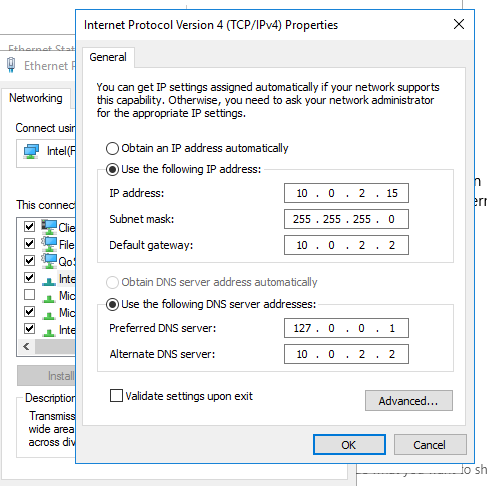
\includegraphics[scale=0.6]{static_ip.png}
\end{figure}

Después de esta configuración, mediante la herramienta de \textit{Server Manager} se han realizado las siguientes tareas:
\begin{enumerate}
\item En el primer menú de\textit{ Configure this local server} se ha cambiado el nombre del servidor local a UOC1.
\item En el segundo menú se han instalado las aplicaciones mencionadas en la Figura 2.
\item Una vez instalado el Active Directory, se puede crear un bosque llamado uoc.local con contraseña de mismas características que el administrador (9 carácteres, minúsculas, mayúsculas y algún número).
\item El sistema pide que se reinicie para la correcta configuración.
\end{enumerate}

\begin{figure}[h!]
\centering
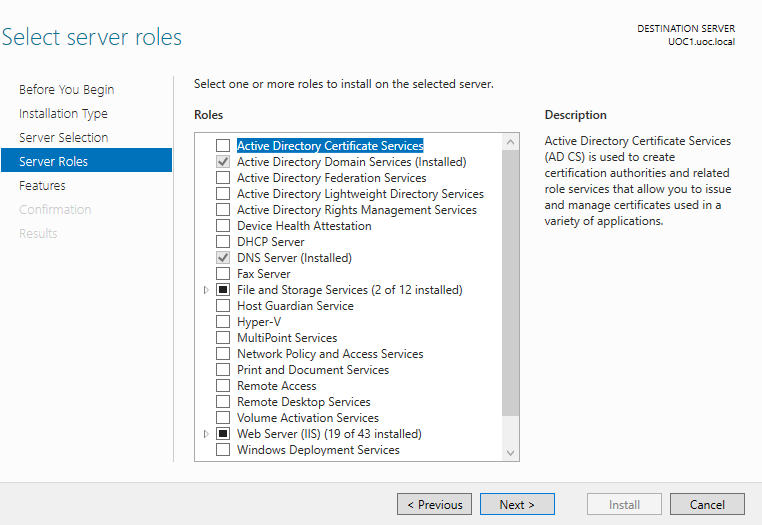
\includegraphics[scale=0.4]{services.png}
\end{figure}

\subsection{}
Tanto el usuario como el grupo se han creado a través del método tradicional de gestión de usuarios de Windows: Computer Management / System Tools / Local Users and Groups / Users \& Groups:\\

\begin{figure}[h!]
\centering
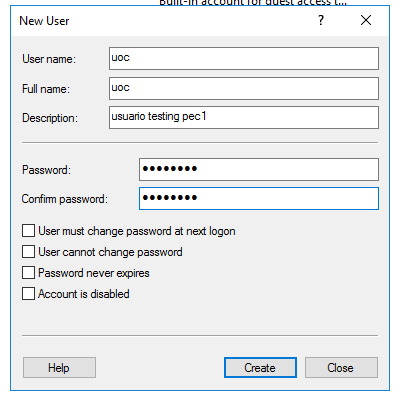
\includegraphics[scale=0.6]{user_create.png}
\end{figure}

La contraseña sigue las mismas características que las del administrador.\\
Posteriormente se ha utilizado la herramienta de Active Directory Users and Computers para asociar el usuario al grupo:
\begin{figure}
\centering
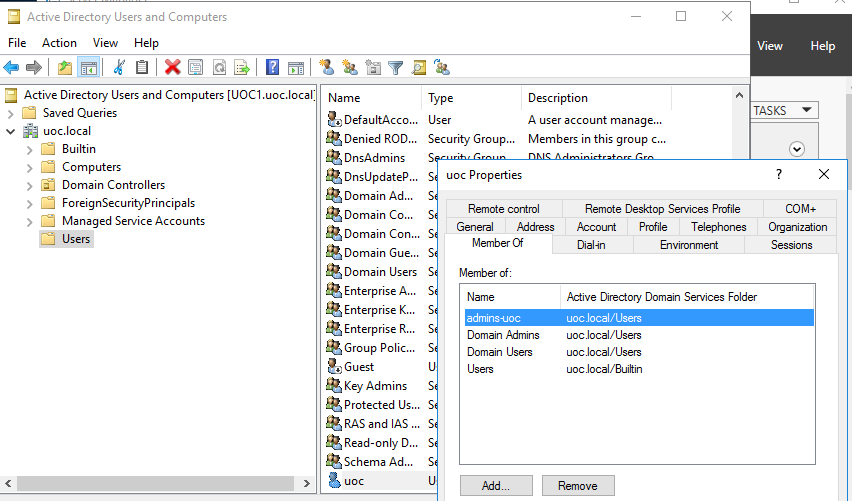
\includegraphics[scale=0.6]{users_and_computers.png}
\end{figure}

\subsection{}

Para este apartado:
\begin{enumerate}
\item Se han creador los directorios usuarios cuyo contenido es uoc dentro de C:
\item En el apartado Properties de la carpeta se cambian los permsisos de acceso en los apartados de Security se conceden permisos al usuario uoc y se eliminan los de los demás
\item En Security también podemos deshabilitar la herencia de permisos para quitarle permisos a los demás usuarios que no sean uoc ni pertencezcan al grupo.
\end{enumerate}
\begin{figure}[h!]
\centering
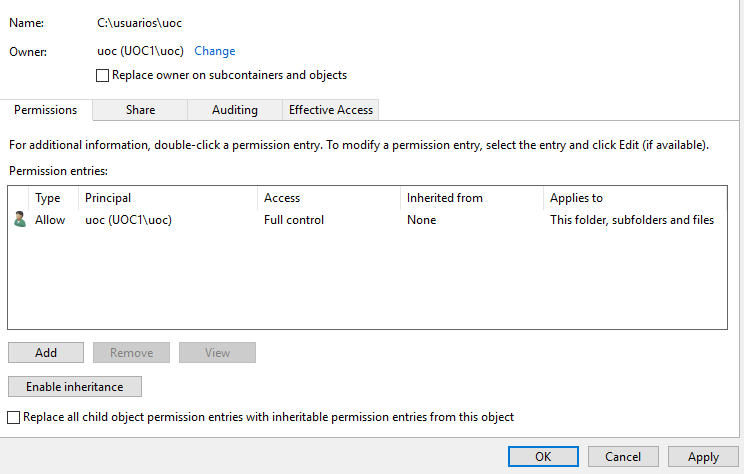
\includegraphics[scale=0.6]{fullcontrol.png}
\end{figure}

Ahora pasamos a usar la aplicación de Active Directory Users and Computers, donde seleccionamos nuevamente a nuestro usuario y en la lengüeta de Profile podemos seleccionar el directorio UOC1\\uoc como unidad Z:

\begin{figure}[h!]
\centering
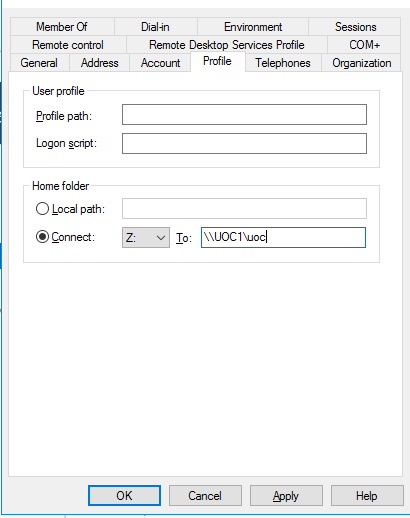
\includegraphics[scale=0.6]{z.png}
\end{figure}

Si nos logueamos como UOC vemos que el directorio se encuentra en nuestro directorio raíz y que somos el único usuario que tiene acceso.

\end{document}